\chapter{Neutrino physics} %%%%%%%%%%%%%%%%%%%%%%%%%%%%%%%%%%%%%%%%%%%%%%%%%%%%%%%%%%%%%%%%%%%%%%%
\label{chap:theory} %%%%%%%%%%%%%%%%%%%%%%%%%%%%%%%%%%%%%%%%%%%%%%%%%%%%%%%%%%%%%%%%%%%%%%%%%%%%%%

Vast numbers of neutrinos pass through everything around us every second, each one incredibly
unlikely even to interact once. Nearly a century since they were first proposed, neutrinos have
now conclusively been proven to undergo oscillations between their different flavours. This
discovery has opened the door to physics beyond that initially conceived within the Standard
Model, which may reveal new, fundamental insights into the universe. This chapter aims to outline
the historical context, theoretical background and open questions surrounding the neutrino.

\section{A history} %%%%%%%%%%%%%%%%%%%%%%%%%%%%%%%%%%%%%%%%%%%%%%%%%%%%%%%%%%%%%%%%%%%%%%%%%%%%%%
\label{sec:theory_history} %%%%%%%%%%%%%%%%%%%%%%%%%%%%%%%%%%%%%%%%%%%%%%%%%%%%%%%%%%%%%%%%%%%%%%%

\subsection{Discovery of the neutrinos} %%%%%%%%%%%%%%%%%%%%%%%%%%%%%%%%%%%%%%%%%%%%%%%%%%%%%%%%%%
\label{sec:theory_history_neutrinos} %%%%%%%%%%%%%%%%%%%%%%%%%%%%%%%%%%%%%%%%%%%%%%%%%%%%%%%%%%%%%

In the early 20th century, beta decays were assumed to follow the simple two-body process,
$A\rightarrow B + e$, where nuclei spontaneously emit a single electron.  The ejected electron was
thought to have discrete kinetic energy, to conserve both energy and angular momentum, defined by
the difference in binding energies between the initial and final nuclei states. However, in 1914,
J. Chadwick instead measured a continuous electron energy spectrum~\cite{chadwick1914}, placing
this theory in doubt.

W. Pauli proposed a `desperate solution' to this paradox in 1930~\cite{pauli1930}. If a light,
neutrally charged, spin $1/2$ particle was also produced, the continuous energy distribution could
be explained. Initially, this mysterious new particle was named the `neutron'. However, to avoid
confusion with the heavy baryon of the same name discovered in 1932, E. Fermi renamed it the
`neutrino' when he formalised beta decay in 1934~\cite{fermi1934}.

The following month, H. Bethe and R. Peierls~\cite{bethe1934} used Fermi's work to estimate the
cross-section of the inverse beta decay process:
\begin{equation} % INVERSE BETA DECAY EQUATION %
    \bar{\nu} + p^{+} \rightarrow n + e^{+}.
    \label{eq:inverse_beta_decay}
\end{equation}
An upper limit of $10^{-44} \mathrm{cm}^2$ was calculated, an incredibly small value, leading them
to declare `there is no practically possible way of observing the neutrino.' This statement hinted
at the vast difficulties experimentalists would face hunting down and measuring the neutrino in
the years to come.

After an initial tentative identification if 1953, F. Reines and C. Cowan made the first confirmed
observation of the neutrino in 1956~\cite{cowan1956}. Electron antineutrinos produced within the
Savannah River Plant nuclear reactor were detected via the inverse beta decay process outlined in
Eq.~\ref{eq:inverse_beta_decay}. In an underground room of the reactor building, A `club-sandwich'
detector of three 1500 litre liquid scintillator tanks and two 200 litre cadmium doped water
target tanks, was constructed. A total of 330 photomultiplier tubes then measured the two
successive characteristic signals for the interaction, allowing for the rejection of the sizeable
cosmic ray background. Firstly, a prompt positron annihilation, followed shortly afterwards by a
gamma-ray burst from the neutron capture.

A second distinct neutrino, the muon neutrino was discovered in 1962 at the Alternating Gradient
Synchrotron (AGS) at Brookhaven~\cite{danby1962}. Protons from the AGS beam incident upon a fixed
target produced charged pions. These would then decay into a beam of muons and neutrinos. After
passing through steel and lead absorbers to remove the muons, neutrino interactions were detected
in a series of spark chambers. If only a single neutrino existed, both interactions
\begin{equation} % BROOKHAVEN DECAY EQUATIONS %
    \nu+p^{+}\rightarrow\mu^{+}+n \\
    \nu+p^{+}\rightarrow e^{+}+n
\end{equation}
would be expected to occur at the same rate. However, only muons, identified by a single long
track were detected, confirming the existence of the muon neutrino. Not only was this experiment
the first to construct and use an artificial neutrino beam, but it also won the 1988 Nobel prize.

The $Z^{0}$ and $W^{\pm}$ bosons, were discovered at the Super Proton Synchrotron at CERN in
1983~\cite{arnison1983_z,arnison1983_w}. Crucially, as $Z^{0}$ bosons were expected to decay to
neutrinos, measurements made to the decay width could strongly constrain the number of neutrino
flavours. The ALEPH, DELPHI, L3 and OPAL experiments at the LEP $e^{+}e^{-}$ collider in the 1990s
made such precise measurements, indicating that the number of light active neutrino flavours to be
$2.984\pm0.008$~\cite{electroweak2006}, see Fig.~\ref{fig:z_resonance}.

\begin{figure} % Z-RESONANCE DIAGRAM %
    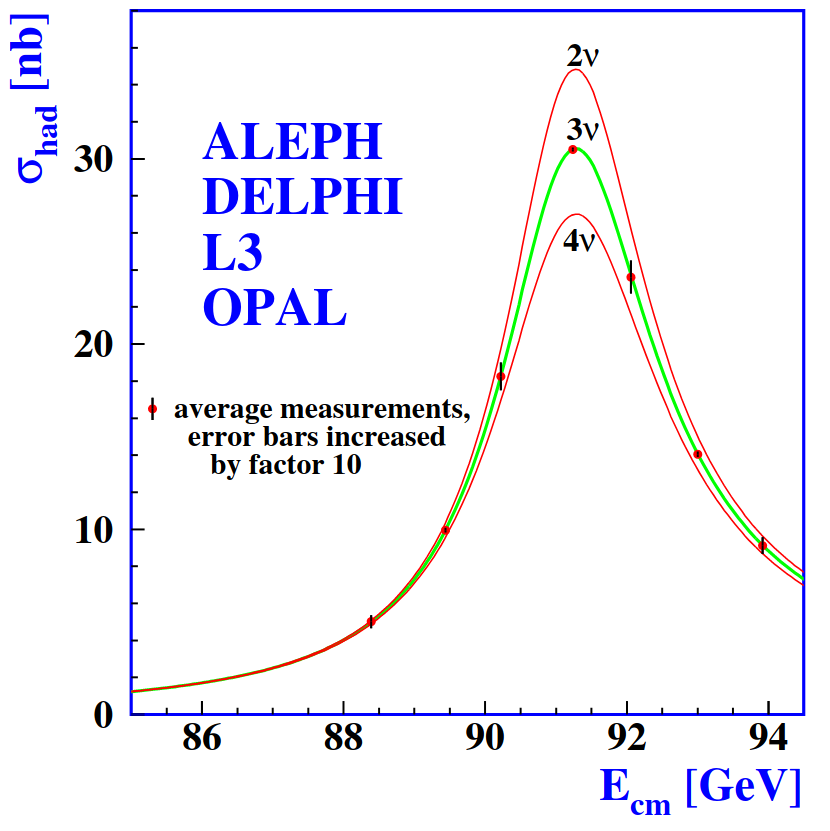
\includegraphics[origin=c,width=0.5\textwidth]{diagrams/3-theory/z_resonance.png}
    \caption[Hadron production cross-section measurements from LEP]
    {Combined hadron production cross-section measurements around the $Z^{0}$ resonance made by
        experiments at LEP. The curves show the predicted cross-section for two, three, and four
        neutrinos. Note how the data fits the three neutrino hypothesis incredibly well. Figure
        taken from Ref.\cite{electroweak2006}.}
    \label{fig:z_resonance}
\end{figure}

Combined with the discovery of the charged tau lepton in 1975~\cite{perl1975}, a third tau
neutrino was likely. The DONUT experiment at Fermilab finally discovered this particle in
2001~\cite{Kodama2001} using \unit{800}{\GeV} ~protons from the Tevatron, completing the trio of
neutrinos we know of today. Any additional neutrinos must either be sterile (do not couple to the
weak force) or have a mass greater than 0.5 $m_{Z}$.

\subsection{Discovery of neutrino oscillations} %%%%%%%%%%%%%%%%%%%%%%%%%%%%%%%%%%%%%%%%%%%%%%%%%%
\label{sec:theory_history_neutrinos} %%%%%%%%%%%%%%%%%%%%%%%%%%%%%%%%%%%%%%%%%%%%%%%%%%%%%%%%%%%%%

At the Homestake mine\footnote{The Homestake mine will be used for the future DUNE experiment
    discussed later} in the 1960s, a large tank, placed 1.5 km underground, was filled with
400000 litres of the dry cleaning fluid, perchloroethylene ($C_{4}Cl_{8}$). Its goal was to
measure the solar electron neutrino flux incident upon the earth via the interaction:
\begin{equation} % HOMESTAKE CHLORINE EQUATION %
    {}^{37}Cl+\nu_{e}\rightarrow{}^{37}Ar+e^{-},
\end{equation} %
allowing the neutrino flux to convert the chlorine contained within the tank to the noble gas
argon. Every few weeks the tank was purged with gaseous helium and the amount of argon generated,
and indirectly the neutrino flux measured.

After analysis, the number of electron neutrino interactions per ${}^{37}Cl$, per second was found
to be no greater than 3~\cite{davis1968}. When compared to the predictions made by the Standard
Solar Model ranging between 4.4 and 22~\cite{bahcall1968}, a deficit was observed. Dubbed the
`solar neutrino problem', it was initially believed to be due to an unexplained experimental flaw.
However, other experiments, such as the water Cherenkov Kamiokande II~\cite{hirata1989} and both
the SAGE and GALLEX galium based capture tanks also observed this
discrepancy~\cite{abazov1991,anselmann1994}.

A neutrino deficit was also observed indirectly in the atmospheric sector. Neutrinos generated in
the atmosphere by cosmic rays formed a key background to the Kamiokande and IMD experiments, both
designed to measure proton decay. When evaluating the background, they observed a deficit in the
number of muon neutrinos compared to electron neutrinos~\cite{hirata1988, becker1992}. The
successor to the Kamiokande experiment Super-Kamiokande also measured the same
deficit~\cite{kajita1999}.

The phenomenon of neutrino oscillations was put forward as a solution to this problem. If
neutrinos could change flavour as they propagated, the measured deficits could be explained. The
SNO experiment finally confirmed this in 2001~\cite{ahmad2002}.

The SNO experiment consisted of a 1 kton tank of deuterium (heavy water), equiped with 9500
photomultiplier tubes. Light from three seperate neutrino interaction channels:
\begin{align} % SNO INTERACTIONS EQUATIONS %
    \nu_{i}+e^{-} & \rightarrow \nu_{i}+e^{-} \\
    \nu_{i}+d     & \rightarrow p+n+\nu_{i}   \\
    \nu_{e}+d     & \rightarrow p+p+e^{-}
\end{align}
was measured, where $d$ is the deuterium nucleus. The first and second channels were sensitive to
all three neutrino flavours, but importantly only electron neutrinos could interact via the third
channel. By comparing the rates between the channels, SNO was able to prove to 5.3$\sigma$ that
electron neutrinos had oscillated to other flavours, whilst the total solar neutrino flux remained
constant.

\section{The Standard Model and neutrinos} %%%%%%%%%%%%%%%%%%%%%%%%%%%%%%%%%%%%%%%%%%%%%%%%%%%%%%%
\label{sec:theory_sm} %%%%%%%%%%%%%%%%%%%%%%%%%%%%%%%%%%%%%%%%%%%%%%%%%%%%%%%%%%%%%%%%%%%%%%%%%%%%

The Standard Model of particle physics describes the 17 known fundamental subatomic particles and
the interactions that take place between them. Combining both quantum chromodynamics (describing
the strong force) and electroweak theory (describing the electromagnetic and weak forces), it is a
gauge theory obeying the local gauge symmetries of $U(1) \times SU(2) \times SU(3)$. The particles,
along with their various properties, are outlined in Fig.~\ref{fig:sm}, additionally, all have an
associated anti-particle with the same quantum numbers except opposite electric charge.

\begin{figure} % STANDARD MODEL DIAGRAM %
    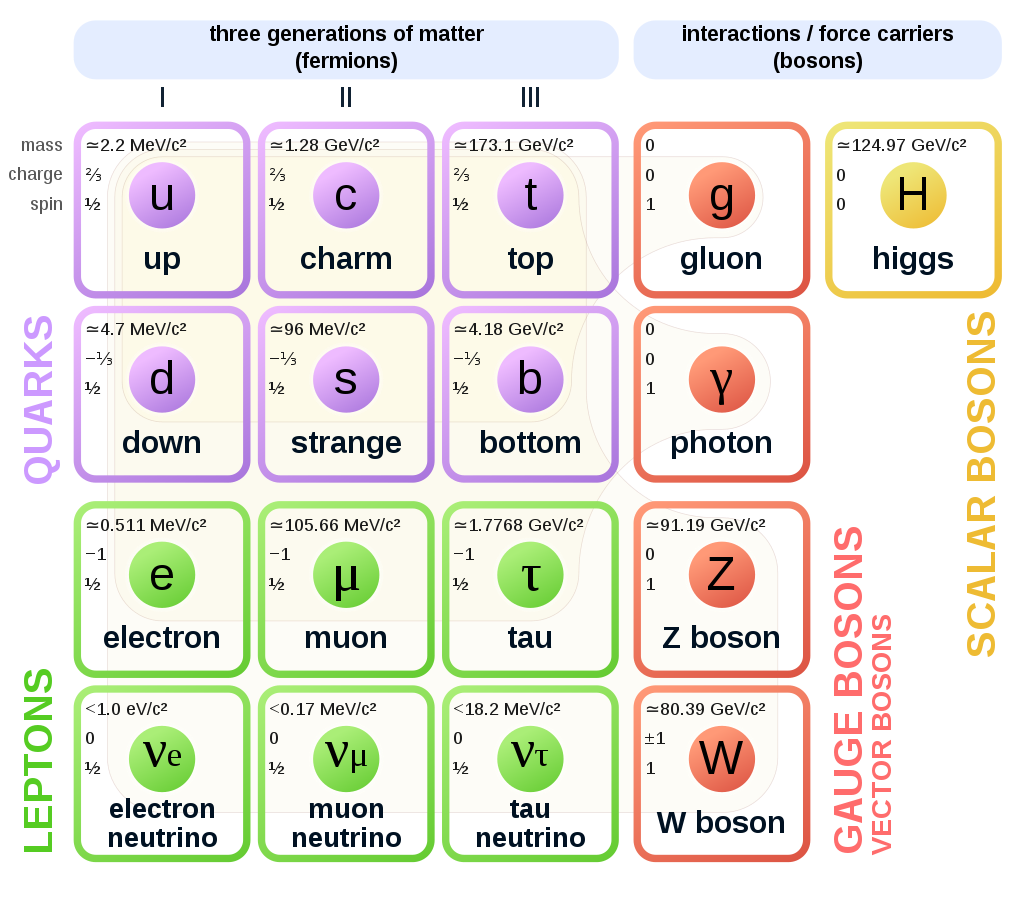
\includegraphics[origin=c,width=0.5\textwidth]{diagrams/3-theory/sm.png}
    \caption[The particles of the Standard Model]
    {The particles of the Standard Model, including the quarks, the leptons and the boson. Figure
        taken from Ref.~\cite{wiki2020}.}
    \label{fig:sm}
\end{figure}

The six quarks and six leptons, all spin 1/2 particles, are named fermions. Further divided into
three generations (or flavours), they make up all the matter content of the universe. The quarks
never exist in a free state and bind together into mesons or baryons, such as pions and protons,
respectively.  Three charged massive particles, the electron, muon and tau and their three
corresponding (initially assumed to be) massless neutrinos, make up the leptons.

The spin 1 gauge bosons carry the electromagnetic, strong and weak forces. The photon carries the
electromagnetic force (affecting all charged particles), the gluons carry the strong force (which
binds the quarks together), and the massive $Z^{0}$ and $W^{\pm}$ carry the weak force. The final
particle, the Higgs, is a massive scalar boson. Via the process of spontaneous symmetry breaking
it provides the mechanism to give all the particles their mass.

Within the Standard Model neutrinos only interact via the weak force, exclusively coupling to the
$Z^{0}$ and $W^{\pm}$ bosons. As the weak interaction maximally violates parity, in that it only
couples to left-handed chiral particles, the original Standard Model only contains left-handed
neutrinos and their corresponding right-handed anti-neutrinos.

Although neutrinos were initially thought to be massless, and no direct detection of their mass
has been made, it is now believed that neutrinos are massive (albeit very light) particles. This
is due to the substantial amount of evidence in support of neutrino oscillations, which require
three distinct neutrino mass states, implying at least two are non-zero.

Cosmological observations of the cosmic microwave background currently provide the best limit on
the combined sum of the neutrino masses at $\sum m_{\nu} < 0.12~\eV$~\cite{planck2018}; however,
this is strongly model-dependent. The KATRIN experiment has been able to make model-independent
direct measurements of the upper limit by looking at the energy spectrum of electrons emitted from
beta decay, giving a result of $m_{\nu} < 1.1~\eV$~\cite{aker2019}.

The Standard Model does not strictly rule out neutrino masses and can be generated by one of two
methods. Either, by including right-handed neutrino fields, a Dirac mass term can be added to the
Standard Model lagrangian to introduce the neutrino masses via the usual Higgs mechanism.
Alternatively, if neutrinos are their own anti-particles, a lepton number violating Majorana mass
term can be introduced.

\section{Neutrino oscillations} %%%%%%%%%%%%%%%%%%%%%%%%%%%%%%%%%%%%%%%%%%%%%%%%%%%%%%%%%%%%%%%%%%
\label{sec:theory_oscillations} %%%%%%%%%%%%%%%%%%%%%%%%%%%%%%%%%%%%%%%%%%%%%%%%%%%%%%%%%%%%%%%%%%

B. Pontecorvo, Z. Maki, M. Nakagawa, and S. Sakata developed the theory of neutrino oscillations
in the 1960s~\cite{maki1962, pontecorvo1967, pontecorvo1969}. Fundamentally, it is a manifestation
of the phenomenon of quantum interference. If neutrinos are massive, their mass eigenstates are
not necessarily the same as their weakly interacting flavour eigenstates. Instead, the flavour
states are a superposition of the three separate mass states, each propagating as distinct waves
evolving differently with time.

As a direct consequence of this, if a neutrino is created with a specific flavour $\alpha$, its
flavour composition will change with time, such that it may later be detected as having a flavour
$\beta$. The probability of this change is found to be periodic (hence oscillations), and depend
on the neutrino energy, the propagation distance and a rotational mixing matrix.

\subsection{Neutrino mixing} %%%%%%%%%%%%%%%%%%%%%%%%%%%%%%%%%%%%%%%%%%%%%%%%%%%%%%%%%%%%%%%%%%%%%
\label{sec:theory_oscillations_mixing} %%%%%%%%%%%%%%%%%%%%%%%%%%%%%%%%%%%%%%%%%%%%%%%%%%%%%%%%%%%

The mixing between the flavour eigenstates $\ket{\nu_{\alpha}}$, where $\alpha=e,\mu,\tau$ and the
mass eigenstates $\ket{\nu_{k}}$, $k=1,2,3$, is described by the Pontecorvo-Maki-Nakagawa-Sakara
(PMNS) matrix $U$, such that,
\begin{equation} % FLAVOUR AS MASS EQUATION %
    \ket{\nu_{\alpha}}=\sum_{k}^{3}U_{\alpha k}^{*}\ket{\nu_{k}},
\end{equation}
and vice-versa,
\begin{equation} % MASS AS FLAVOUR EQUATION %
    \ket{\nu_{k}}=\sum_{\alpha}^{3}U_{\alpha k}\ket{\nu_{\alpha}}.
\end{equation}
The PMNS matrix is a unitary, complex, $3\times3$ matrix, similar to the Cabibbo-Kobayashi-Maskawa
(CKM) matrix for quark mixing, and has the form,
\begin{gather} % PMNS MATRIX SIMPLE %
    \begin{pmatrix}
        \ket{\nu_{e}}   \\
        \ket{\nu_{\mu}} \\
        \ket{\nu_{\tau}}
    \end{pmatrix}
    =
    \begin{pmatrix}
        U_{e1}     & U_{e2}     & U_{e3}     \\
        U_{\mu 1}  & U_{\mu 2}  & U_{\mu 3}  \\
        U_{\tau 1} & U_{\tau 2} & U_{\tau 3}
    \end{pmatrix}
    \begin{pmatrix}
        \ket{\nu_{1}} \\
        \ket{\nu_{2}} \\
        \ket{\nu_{3}}
    \end{pmatrix}.
\end{gather} %
Three mixing angles and six complex phases can generally describe a $3\times3$ matrix such as
this. However, the majority of these phases can be removed without affecting any physical
processes. This leaves three mixing angles $\theta_{12}$, $\theta_{23}$, $\theta_{13}$ and a
single phase $\delta$ which if non-zero produces CP violation and so is commonly named
$\delta_{CP}$.

With $s_{ij}=\sin \theta_{ij}$ and $c_{ij}=\cos \theta_{ij}$, the standard parameterisation of
$U$ assuming neutrinos are Dirac particles is given by,
\begin{align} % DIRAC PMNS MATRIX FULL %
    \mathrm{U} & =
    \begin{pmatrix}
        1 & 0       & 0      \\
        0 & c_{23}  & s_{23} \\
        0 & -s_{23} & c_{23}
    \end{pmatrix}
    \begin{pmatrix}
        c_{13}                   & 0 & s_{13}e^{-i\delta_{CP}} \\
        0                        & 1 & 0                       \\
        -s_{13}e^{-i\delta_{CP}} & 0 & c_{13}
    \end{pmatrix}
    \begin{pmatrix}
        c_{12}  & s_{12} & 0 \\
        -s_{12} & c_{12} & 0 \\
        0       & 0      & 1
    \end{pmatrix}
    \\
               & =
    \begin{pmatrix}
        c_{12}c_{13}
         & s_{12}c_{13}
         & s_{13}e^{-i\delta_{CP}}                          \\
        -s_{12}c_{23}-c_{12}s_{23}s_{13}e^{i\delta_{CP}}
         & c_{12}c_{23}-s_{12}s_{23}s_{13}e^{i\delta_{CP}}
         & s_{23}c_{13}                                     \\
        s_{12}s_{23}-c_{12}c_{23}s_{13}e^{i\delta_{CP}}
         & -c_{12}s_{23}-s_{12}c_{23}s_{13}e^{i\delta_{CP}}
         & c_{23}c_{13}
    \end{pmatrix}.
\end{align} %
The three-component representation separates the regimes that are commonly explored by different
types of experiment. These are, $\theta_{23}$ for atmospheric, $\theta_{12}$ for solar, and
$\theta_{13}$ for reactor $\nu_{e}$ disappearance or beam $\nu_{e}$ appearance. These three
regimes will be discussed in detail in the following chapter.

If neutrinos are instead Majorana in nature two additional phases $\alpha_{21}$ and $\alpha_{31}$
are required, such that the mixing matrix needs to be multiplied by,
\begin{align} % MAJORANA DIAGONAL PMNS EQUATION %
    \mathrm{diag}(1, e^{\frac{i\alpha_{21}}{2}}, e^{\frac{i\alpha_{31}}{2}}).
\end{align} %
Note that both these phases lie on the diagonal and hence have no effect on the oscillations.

\subsection{Oscillations in vacuum} %%%%%%%%%%%%%%%%%%%%%%%%%%%%%%%%%%%%%%%%%%%%%%%%%%%%%%%%%%%%%%
\label{sec:theory_oscillations_vacuum} %%%%%%%%%%%%%%%%%%%%%%%%%%%%%%%%%%%%%%%%%%%%%%%%%%%%%%%%%%%

As the neutrino mass states are eigenstates of the hamiltonian with energy eigenvalues $E_{k}$:
\begin{equation} % HAMILTONIAN EQUATION %
    H \ket{\nu_{k}} = E_{k} \ket{\nu_{k}},
    \label{eq:hamiltonian}
\end{equation}
their time evolution is described by the Schr$\mathrm{\ddot{o}}$dinger equation. This can be used
to determine how the neutrino flavour state, evolves with time, such that,
\begin{equation} % TIME EVOLUTION EQUATION %
    \ket{\nu_{\alpha}(t)}=\sum_{k}^{3}U_{\alpha k}^{*}e^{-iE_{k}t}\ket{\nu_{k}}.
    \label{eq:time_evolution_1}
\end{equation}

After a time $t$, the probability of finding $\ket{\nu_{\alpha}}$ in the state $\ket{\nu_{\beta}}$
is then given by,
\begin{equation} % TIME EVOLUTION EQUATION %
    P(\nu_{\alpha} \rightarrow \nu_{\beta}, t) = |\braket{\nu_{\beta}|\nu_{\alpha}(t)}|^{2}=
    \abs*{\sum_{k}^{3}U_{\alpha k}^{*}U_{\beta k}e^{-iE_{k}t}}^{2} \\
    =\sum_{k}^{3}\sum_{j}^{3}U_{\alpha k}^{*}U_{\beta k}U_{\alpha j}U_{\beta j}^{*}
    e^{i(E_{k}-E_{j})t}.
    \label{eq:osc_prob_1}
\end{equation}
As neutrinos are ultrarelativistic ($p\simeq E$) the approximation,
\begin{equation} % ENERGY, MASS, MOMENTUM EQUATION %
    E_{k}=\sqrt{\vec{p}_{k}^{\,2}+m_{k}^{2}}\simeq E+\frac{m_{k}^{2}}{2E},
    \label{eq:energy_mass_momentum}
\end{equation}
where $\vec{p}_{k}$ and $m_{k}$ are the neutrino momentum and energy, and $E$ is the neutrino
energy without the mass, can be made. This allows the substitution,
\begin{equation} % ENERGY, MASS, MOMENTUM EQUATION %
    E_{k}-E_{j}\approx\frac{\Delta m_{kj}^{2}}{2E},
    \label{eq:energy_mass_momentum}
\end{equation}
where $\Delta m_{kj}^{2}$ is the squared mass difference (mass splitting) between the $k$ and $j$
mass states. Additionally, the relativistic limit allows the simplification $t = L$, where
$L$ is the distance from neutrino creation to detection. Combined, the oscillation probability
can be written as,
\begin{align} % TIME EVOLUTION EQUATION %
    P(\nu_{\alpha} \rightarrow \nu_{\beta}, t) = \delta_{\alpha\beta} & - 4\sum_{k>j}re(
    U_{\alpha k}^{*}U_{\beta k}U_{\alpha j}U_{\beta j}^{*})\sin^{2}\left(\frac{\Delta
        m_{kj}^{2}L}{4E}\right) \nonumber
    \\  & \pm 2\sum_{k>j}im(
    U_{\alpha k}^{*}U_{\beta k}U_{\alpha j}U_{\beta j}^{*})\sin\left(\frac{\Delta
        m_{kj}^{2}L}{4E}\right),
    \label{eq:osc_prob_2}
\end{align}
where the last term has a positive sign for neutrinos and a negative sign for anti-neutrinos.

From inspecting Eq.~\ref{eq:osc_prob_2}, the superposition of mass eigenstates drives the
oscillation of the flavour state. A set experimental location and neutrino source define a
constant $L/E$. The period of oscillations is thus determined by the squared mass difference
between the flavour states $\Delta m_{kj}^{2}$.  Furthermore, the amplitude of the oscillation
arises from the elements of the PMNS matrix.

\subsection{Oscillations in matter} %%%%%%%%%%%%%%%%%%%%%%%%%%%%%%%%%%%%%%%%%%%%%%%%%%%%%%%%%%%%%%
\label{sec:theory_oscillations_matter} %%%%%%%%%%%%%%%%%%%%%%%%%%%%%%%%%%%%%%%%%%%%%%%%%%%%%%%%%%%

As neutrinos propagate through matter, they undergo coherent forward scattering with nucleons.
These interactions do not change the neutrino state or momentum, but they do impart an interaction
potential onto the neutrinos. Two types of interaction can take place, either through the exchange
of a $Z^{0}$ in a neutral current (NC) interaction, or a $W^{\pm}$ in a charged current (CC)
process. The two interaction potentials are given by,
\begin{align} % EFFECTIVE POTENTIAL EQUATION %
    V_{NC} & = \frac{\pm 1}{\sqrt{2}}G_{F}n_{n} \\
    V_{CC} & = \pm\sqrt{2}G_{F}n_{e},
\end{align}
were $n_{n}$ and $n_{e}$ are the number density of neutrons and electrons in the medium
respectively and $G_{F}$ is Fermi's constant. The sign of the potential is positive for neutrinos
and negative for anti-neutrinos.

Crucially, as matter is full of electrons, but empty of muons or taus, only electron neutrinos can
interact via the CC channel as shown in Fig.~\ref{fig:coherent_scattering}. As a consequence, only
electron neutrinos are affected by the $V_{CC}$ potential, while all are affected by the $V_{NC}$
potential. When quantitatively applied as an additional potential to the vacuum hamiltonian, a
resonance term is introduced which significantly modifies the vacuum oscillation probabilities.
This effect is know as the Mikheev, Smirnov and Wolfenstein (MSW) effect~\cite{wolfenstein1978,
    mikheev1986}.

It is important to note two things. Firstly, a difference between neutrinos and antineutrinos is
introduced by the $\pm$ in the $V_{CC}$ potential. Secondly, the modified oscillation probability
is found to be non-symmetric with respect to the sign of the $\Delta m^{2}$ parameters.

\begin{figure} % NUEL COHERENT SCATTERING DIAGRAM %
    \feynmandiagram[vertical'=a to b] {
    i1 [particle=\(\nu_{e}\)]-- [fermion] a-- [fermion] f1 [particle=\(e^{-}\)],
    a -- [boson,edge label=\(W^{\pm}\)] b,
    i2 [particle=\(e^{-}\)]-- [fermion] b-- [fermion] f2 [particle=\(\nu_{e}\)],
    };
    \caption[$\nu_{e}$ coherent scattering Feynman diagram]
    {Feynman diagram of coherent scattering of a $\nu_{e}$ on an electron in a charged current
        process.}
    \label{fig:coherent_scattering}
\end{figure}

\section{Open Questions} %%%%%%%%%%%%%%%%%%%%%%%%%%%%%%%%%%%%%%%%%%%%%%%%%%%%%%%%%%%%%%%%%%%%%%%%%
\label{sec:theory_questions} %%%%%%%%%%%%%%%%%%%%%%%%%%%%%%%%%%%%%%%%%%%%%%%%%%%%%%%%%%%%%%%%%%%%%

There are still clear and open questions regarding the various parameters of the PMNS matrix.
After briefly outlining them below, discussion of how current and future experimental efforts
aim to resolve these questions will be outlined in the following chapter.

\subsection[Octant of theta 23]{Octant of $\theta_{23}$} %%%%%%%%%%%%%%%%%%%%%%%%%%%%%%%%%%%%%%%%%%
\label{sec:theory_questions_octant} %%%%%%%%%%%%%%%%%%%%%%%%%%%%%%%%%%%%%%%%%%%%%%%%%%%%%%%%%%%%%%

It is known that the mixing angle $\theta_{23}$ is non-zero and large. Initially thought to be
maximal such that, $\theta_{23}=\pi/4=45^{\circ}$, we now know that this is not the case. However,
it is still unclear if $\theta_{23}<45^{\circ}$ or $\theta_{23}>45^{\circ}$, commonly referred to
as the octant. Although easily measured be studying $\nu_{\mu}$ disappearance, a degeneracy in the
oscillation probability removes the ability to determine the octant. $\nu_{e}$ appearance,
however, contains an oscillation term allowing for the octant to be resolved, but an exploration
of this channel is yet to produce a significant result.

\subsection{Mass hierarchy} %%%%%%%%%%%%%%%%%%%%%%%%%%%%%%%%%%%%%%%%%%%%%%%%%%%%%%%%%%%%%%%%%%%%%%
\label{sec:theory_questions_hierarchy} %%%%%%%%%%%%%%%%%%%%%%%%%%%%%%%%%%%%%%%%%%%%%%%%%%%%%%%%%%%

Neutrino oscillation experiments allow us to measure the mass squared differences between the
neutrino mass states. The value of $\Delta m_{21}^2$ has been measured by solar neutrino
experiments and is known to be small and positive. Meaning that $m_{2}>m_{1}$ where $m_{1}$ is
defined to be the dominant mass state of the electron neutrino. However, the sign of $\Delta
    m_{32}^2$ is currently unknown. This allows for two possible scenarios, either $m_1<m_2<m_3$,
known as normal hierarchy, or $m_3<m_1<m_2$, known as inverted hierarchy. Both are illustrated
in Fig.~\ref{fig:hierarchy}.

Oscillations in vacuum are not sensitive to the sign of the $\Delta m^{2}$ parameters. However,
matter effects allow for the sign to be determined. Resolving this ambiguity will significantly
improve the ability of experiments to both determine the value of $\delta_{CP}$ and discover if
neutrinos are Dirac or Majorana in nature.

\begin{figure} % MASS HIERARCHY DIAGRAM %
    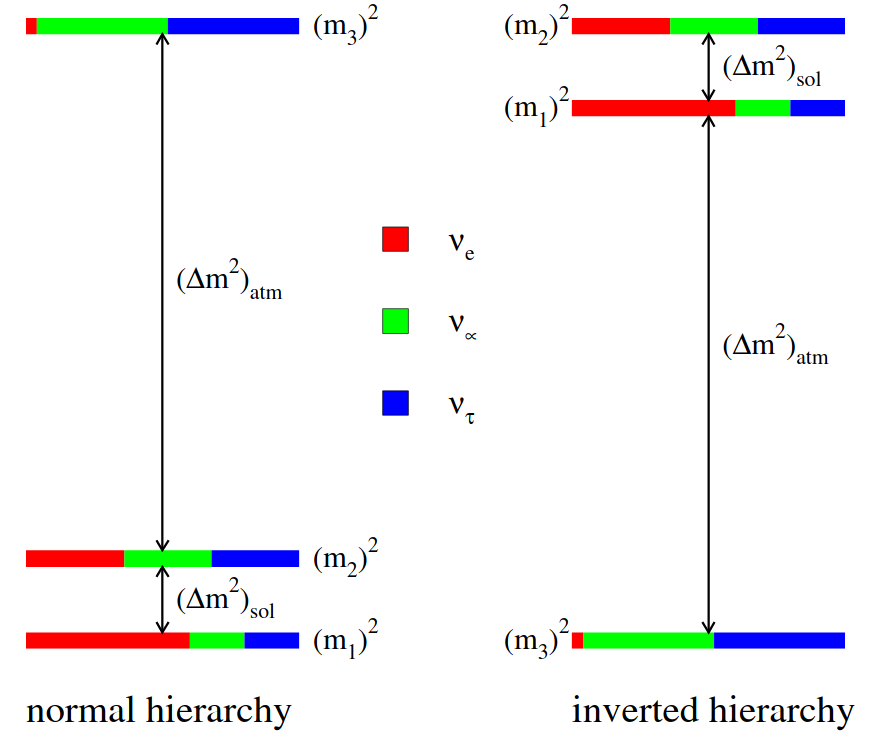
\includegraphics[origin=c,width=0.5\textwidth]{diagrams/3-theory/hierarchy.png}
    \caption[Illustration of the two possible mass hierarchies]
    {Illustrated diagram of the two possible mass hierarchies. The atmospheric (atm) and solar
        (sol) naming convention is used for the mass differences. The sign of
        $\Delta m_{21}^{2}$ is small and positive, while the sign of $\Delta m_{32}^{2}$ is
        unknown. Figure taken from Ref.\cite{gouvea2013}.}
    \label{fig:hierarchy}
\end{figure}

\subsection{CP-violation} %%%%%%%%%%%%%%%%%%%%%%%%%%%%%%%%%%%%%%%%%%%%%%%%%%%%%%%%%%%%%%%%%%%%%%%%
\label{sec:theory_questions_cp} %%%%%%%%%%%%%%%%%%%%%%%%%%%%%%%%%%%%%%%%%%%%%%%%%%%%%%%%%%%%%%%%%%

The current level of CP violation observed in the quark sector does not fully explain the
matter-antimatter asymmetry of the universe. However, if CP violation is shown to exist in the
leptonic sector, leptogenesis models of the early universe allow this to go some way to resolving
the issue. The PMNS matrix allows for
$P(\nu_{\alpha}\rightarrow\nu_{\beta}) \neq P(\bar{\nu_{\alpha}}\rightarrow\bar{\nu_{\beta}})$,
when $\delta_{CP}$ is not 0 or $\pi$. The most promising channel for this measurement is $\nu_{e}$
appearance from a $\nu_{\mu}$ neutrino source, where the oscillation probabilities change
significantly, as shown in Fig.~\ref{fig:osc_cp_probs}.

\begin{figure} % OSCILLATION CP PROBS DIAGRAM %
    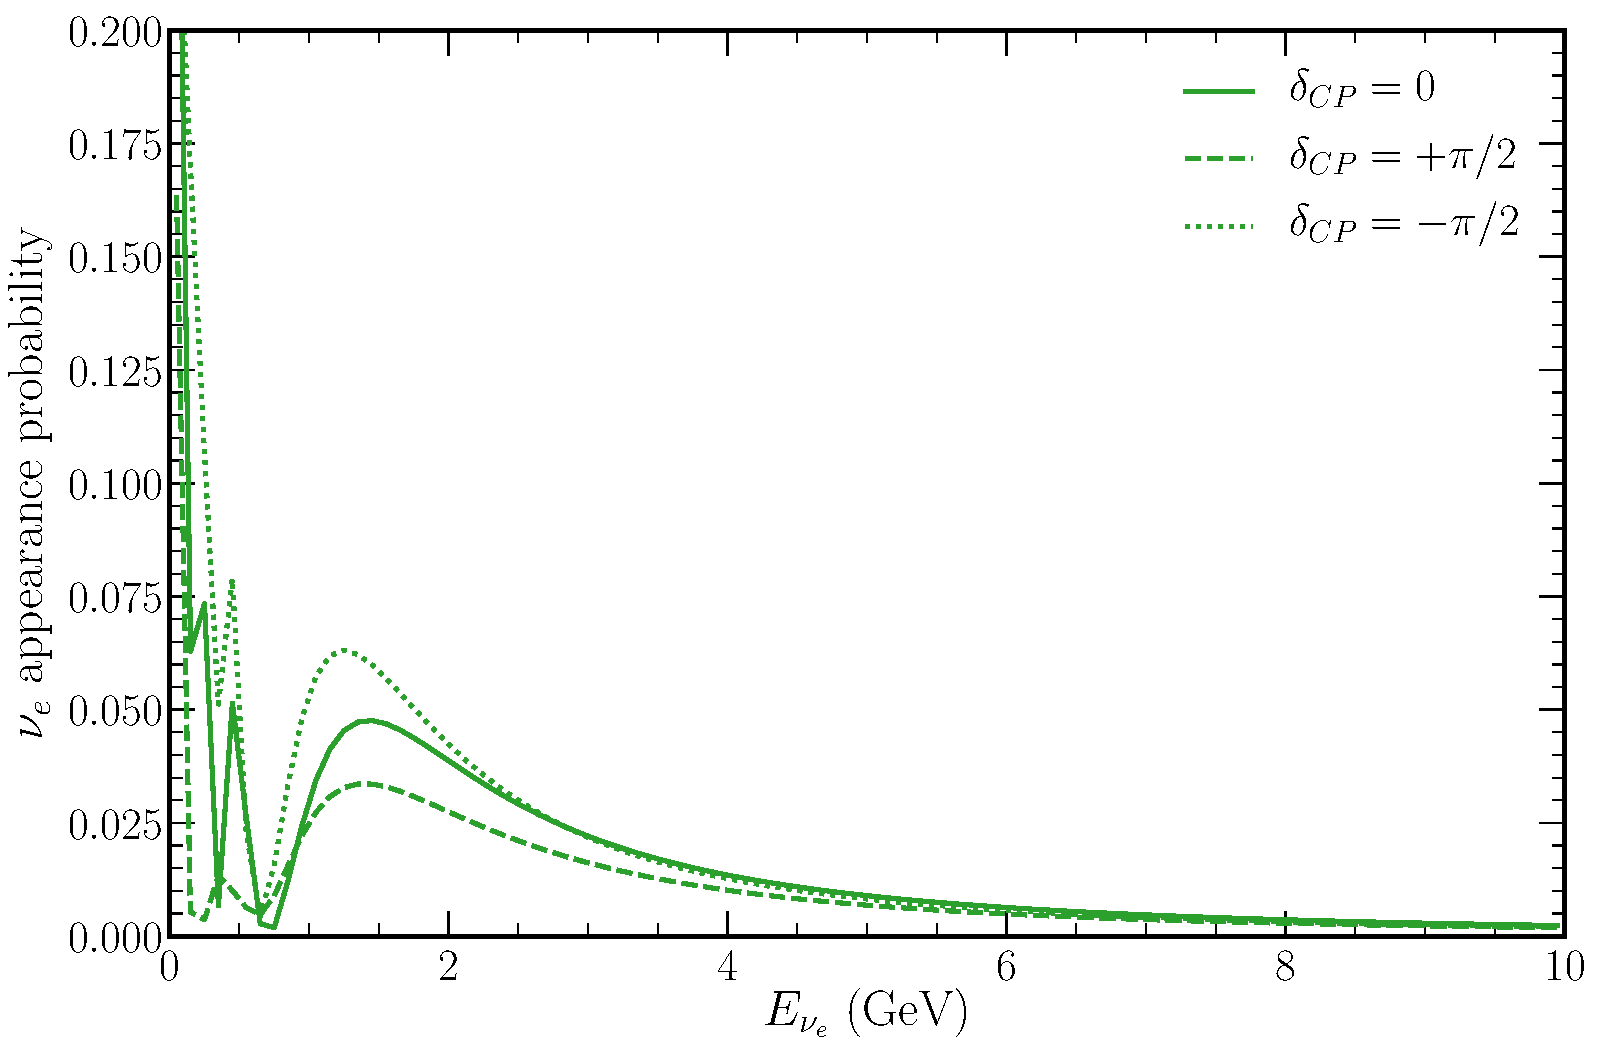
\includegraphics[origin=c,width=0.7\textwidth]{diagrams/7-cvn/chipsnet/explore_osc_cp_probs.pdf}
    \caption[$\nu_{e}$ appearance probability for different $\delta_{CP}$ values]
    {Appearance probability of $\nu_{e}$ oscillating from $\nu_{\mu}$ at $L=712$ km. The
        oscillations are show for three different values of $\delta_{CP}$.}
    \label{fig:osc_cp_probs}
\end{figure}

\section{Oscillation parameter values} %%%%%%%%%%%%%%%%%%%%%%%%%%%%%%%%%%%%%%%%%%%%%%%%%%%%%%%%%%%
\label{sec:theory_summary} %%%%%%%%%%%%%%%%%%%%%%%%%%%%%%%%%%%%%%%%%%%%%%%%%%%%%%%%%%%%%%%%%%%%%%%

DIAGRAM: Table of the current best fit oscillation parameters